\chapter{The 2D Fourier Transform and Image Filtering}

In the last chapter we learned to see an image as a two-dimensional signal: a
function $f(x,y)$ that assigns a brightness to every point on a grid. That is a
complete picture, but it is a picture in the \emph{spatial} domain -- it tells you
\emph{where} the bright and dark patches sit. This chapter learns the other half
of the story. Every image can also be written as a sum of two-dimensional waves,
ripples of brightness that march across the picture in some direction at some
spacing. The recipe of those waves is the \emph{2D Fourier transform}, and once
you can read it the toolbox opens up: blur and sharpen with fine
control, remove periodic interference, detect orientation, compress a photo to a
tenth of its size, and see why every camera and every eye is, at bottom, a
frequency-limited device.

Everything we built in one dimension carries over. A 1D signal was a sum of
sinusoids $e^{\jj 2\pi f t}$ that differ in \emph{frequency} -- how fast they
wiggle. A 2D image is a sum of sinusoids $e^{\jj 2\pi (ux + vy)}$ that differ in
two numbers: how fast they wiggle \emph{and} in which \emph{direction}. That extra
degree of freedom -- direction -- is the only genuinely new idea in the whole
chapter. Hold onto it.

\begin{focusbox}
By the end you should be able to look at an image and predict roughly where its
energy sits in the 2D spectrum (smooth regions near the center, edges and texture
out at the rim, repeating patterns as bright dots), design a low-pass or high-pass
filter by reaching into that spectrum and reshaping it, and know exactly why a
$3\times3$ blur kernel and a $1\times3$-then-$3\times1$ pair of kernels can give
the identical result for a fraction of the work.
\end{focusbox}

\section{Two-dimensional waves: the new basis}
\label{ch31:2d-waves}

In one dimension the building block was a phasor $e^{\jj 2\pi f t}$: a unit vector
spinning at frequency $f$. Its real part, $\cos(2\pi f t)$, is a wave that
oscillates as you move along the single time axis.

In two dimensions we have two axes, $x$ and $y$. The natural building block is

\begin{equation}
b_{u,v}(x,y) \;=\; e^{\jj 2\pi (u x + v y)}
\;=\; \cos\!\big(2\pi(ux+vy)\big) \;+\; \jj\,\sin\!\big(2\pi(ux+vy)\big).
\label{ch31:basis}
\end{equation}

Look at the real part, $\cos(2\pi(ux+vy))$. Its value depends only on the
combination $ux+vy$. The set of points where $ux+vy$ is constant is a
\emph{straight line} -- a level set -- and as you cross those lines the cosine runs
through its cycle. So $b_{u,v}$ is a corrugated sheet: parallel ridges and
troughs of brightness, like a sheet of corrugated iron viewed from above.

Two numbers control that sheet.

\begin{itemize}
\item The \textbf{direction} of the ripples is set by the vector
$(u,v)$. The ridges run \emph{perpendicular} to $(u,v)$; the brightness changes
fastest \emph{along} $(u,v)$.
\item The \textbf{spatial frequency} -- how tightly the ridges are packed -- is the
length $\sqrt{u^2+v^2}$. A large length means closely spaced ripples (fine
detail); a small length means broad, lazy ripples (smooth shading). The spacing
between ridges, the wavelength, is $1/\sqrt{u^2+v^2}$.
\end{itemize}

\begin{intuitionbox}
A 1D frequency was a single number on a line. A 2D spatial frequency is a
\emph{vector} $(u,v)$ in a plane. Its \emph{length} is ``how fine'' and its
\emph{angle} is ``which way.'' Everything strange about 2D Fourier -- diagonal
streaks in the spectrum, the way a vertical fence makes horizontal dots -- is just
this vector wearing a disguise. When in doubt, draw the arrow $(u,v)$ and remember
the ripples run across it.
\end{intuitionbox}

Figure~\ref{ch31:fig-grating} shows three of these gratings. Notice that rotating
$(u,v)$ rotates the stripes, and lengthening $(u,v)$ squeezes them together.

\begin{figure}[H]
\centering
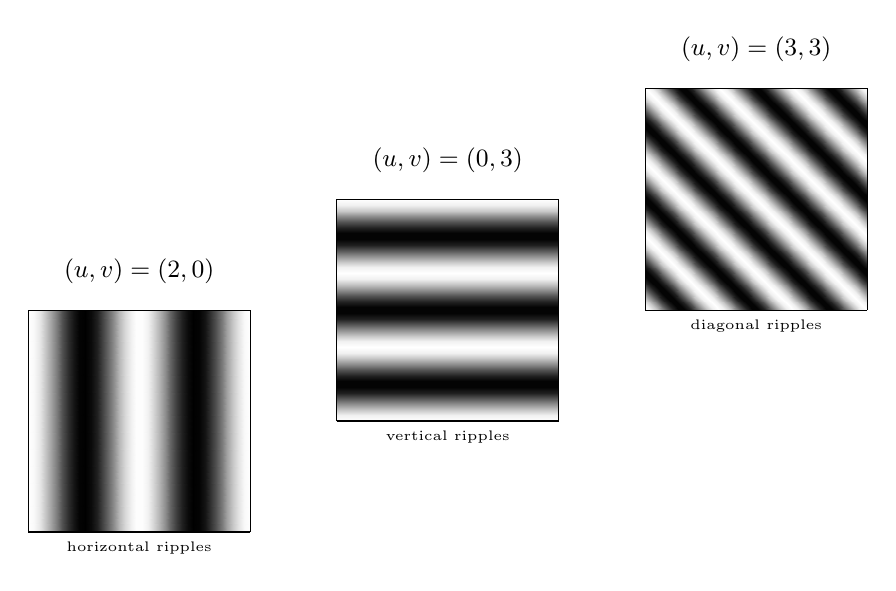
\begin{tikzpicture}
\begin{axis}[name=A,width=4.4cm,height=4.4cm,enlargelimits=false,
  axis on top,xtick=\empty,ytick=\empty,
  title={\small $(u,v)=(2,0)$},xlabel={\tiny horizontal ripples},
  domain=0:1,y domain=0:1,view={0}{90},
  colormap/blackwhite,point meta min=-1,point meta max=1]
\addplot3[surf,shader=interp,samples=40] {cos(deg(2*pi*(2*x+0*y)))};
\end{axis}
\begin{axis}[name=B,at={(A.east)},xshift=1.1cm,width=4.4cm,height=4.4cm,
  enlargelimits=false,axis on top,xtick=\empty,ytick=\empty,
  title={\small $(u,v)=(0,3)$},xlabel={\tiny vertical ripples},
  domain=0:1,y domain=0:1,view={0}{90},
  colormap/blackwhite,point meta min=-1,point meta max=1]
\addplot3[surf,shader=interp,samples=40] {cos(deg(2*pi*(0*x+3*y)))};
\end{axis}
\begin{axis}[name=C,at={(B.east)},xshift=1.1cm,width=4.4cm,height=4.4cm,
  enlargelimits=false,axis on top,xtick=\empty,ytick=\empty,
  title={\small $(u,v)=(3,3)$},xlabel={\tiny diagonal ripples},
  domain=0:1,y domain=0:1,view={0}{90},
  colormap/blackwhite,point meta min=-1,point meta max=1]
\addplot3[surf,shader=interp,samples=40] {cos(deg(2*pi*(3*x+3*y)))};
\end{axis}
\end{tikzpicture}
\caption{Three 2D cosine gratings $\cos(2\pi(ux+vy))$. The frequency vector
$(u,v)$ sets the direction (ripples run perpendicular to it) and the fineness (its
length). These corrugated sheets are the basis from which every image is built.}
\label{ch31:fig-grating}
\end{figure}

\begin{whybox}
Why are these the right building blocks and not, say, little blobs or wavelets?
Because shifting an image must do something \emph{simple}. The deepest fact of
Fourier analysis -- in any number of dimensions -- is that complex exponentials are
the eigenfunctions of shift: slide $b_{u,v}$ by $(a,b)$ and you get the very same
sheet back, multiplied by the constant phase $e^{\jj 2\pi(ua+vb)}$. Nothing else
has that property. Because real-world imaging operations (lenses blurring,
sensors averaging, translations) are shift-invariant, the gratings are the natural
coordinates in which those operations become simple multiplications. We saw this
in 1D for LTI systems; in 2D it is identical, just with two shift directions.
\end{whybox}

\section{The 2D DFT}
\label{ch31:2d-dft}

A digital image is sampled: an $M\times N$ grid of pixels $f[m,n]$, with row index
$m=0,\dots,M-1$ and column index $n=0,\dots,N-1$. The two-dimensional discrete
Fourier transform is the discrete cousin of the projection in
Eq.~\eqref{ch31:basis}:

\begin{equation}
F[k,\ell] \;=\; \sum_{m=0}^{M-1}\sum_{n=0}^{N-1}
f[m,n]\, e^{-\jj 2\pi\left(\frac{k m}{M} + \frac{\ell n}{N}\right)},
\label{ch31:dft2d}
\end{equation}

with the inverse

\begin{equation}
f[m,n] \;=\; \frac{1}{MN}\sum_{k=0}^{M-1}\sum_{\ell=0}^{N-1}
F[k,\ell]\, e^{+\jj 2\pi\left(\frac{k m}{M} + \frac{\ell n}{N}\right)}.
\label{ch31:idft2d}
\end{equation}

Here $k$ indexes vertical frequency (along $m$, the rows) and $\ell$ indexes
horizontal frequency (along $n$, the columns). Each output $F[k,\ell]$ is a complex
number: a magnitude $\abs{F[k,\ell]}$ saying how much of that grating is present,
and a phase $\angle F[k,\ell]$ saying where its ridges sit.

\begin{happeningbox}
$F[k,\ell]$ is the inner product of the image with the grating $b_{k,\ell}$. We are
asking, for each direction and fineness, ``how much does the image look like
\emph{this} corrugated sheet?'' The whole transform is $MN$ such questions, one per
output pixel. The answer to each is a single complex number -- a length and an
angle -- and the inverse transform just adds all those gratings back up, weighted by
those numbers, to rebuild the picture exactly. Nothing is lost: the spectrum is
the image, in different clothes.
\end{happeningbox}

\subsection{The transform separates into rows then columns}
\label{ch31:separable-dft}

Equation~\eqref{ch31:dft2d} looks like a double sum of size $MN$ per output, which
would be $O(M^2N^2)$ operations -- ruinous. But the exponential \emph{factors}:
\[
e^{-\jj 2\pi(\frac{km}{M}+\frac{\ell n}{N})}
= e^{-\jj 2\pi \frac{km}{M}}\; e^{-\jj 2\pi \frac{\ell n}{N}}.
\]
So we can split the work:
\begin{equation}
F[k,\ell] = \sum_{m=0}^{M-1}\underbrace{\left(\sum_{n=0}^{N-1}
f[m,n]\,e^{-\jj 2\pi \frac{\ell n}{N}}\right)}_{\text{1D DFT of row } m}
e^{-\jj 2\pi \frac{km}{M}}.
\label{ch31:rowcol}
\end{equation}
First take the ordinary 1D DFT of every \emph{row}; then take the 1D DFT of every
\emph{column} of the result. (The order does not matter.) Each 1D DFT can use the
FFT from Chapter~9, so the 2D DFT of an $N\times N$ image costs $O(N^2\log N)$, not
$O(N^4)$. This row--column trick is the workhorse behind every image-processing
library.

\begin{whybox}
Why does ``rows then columns'' give the same answer as the full 2D sum? Because the
2D basis is a \emph{product} of a row-basis and a column-basis. The 2D DFT is a
\emph{separable} transform: it is the 1D DFT applied along one axis composed with
the 1D DFT applied along the other. Separability is not a numerical accident; it is
the algebraic shadow of the fact that the plane is a product of two lines.
\end{whybox}

\section{Reading a 2D spectrum}
\label{ch31:reading}

We almost always look at the \emph{magnitude} spectrum $\abs{F[k,\ell]}$, displayed
as an image. Three conventions make it legible.

\begin{enumerate}
\item \textbf{Shift the DC term to the center.} As in 1D, the DFT's frequencies
wrap around: index $0$ is zero frequency, and the highest frequencies sit near the
middle of the index range, with negatives folded to the top end. We
\texttt{fftshift} so that $(0,0)$ -- the average brightness, the ``DC'' term --
lands at the \emph{center} of the displayed image. Then low frequencies cluster at
the center and high frequencies spread to the corners.
\item \textbf{Take a log.} Spectral magnitudes span many orders of magnitude; the
DC term alone dwarfs everything. We display $\log(1+\abs{F})$ so the faint
high-frequency structure becomes visible.
\item \textbf{Ignore the phase at first.} The magnitude tells you \emph{which}
gratings are present and how strongly; the phase tells you \emph{where} they sit.
For building intuition the magnitude is enough -- but never forget the phase is
doing the heavy lifting (see the box below).
\end{enumerate}

Now the payoff -- a vocabulary for reading the picture, summarized in
Figure~\ref{ch31:fig-spectrum}:

\begin{itemize}
\item \textbf{Center bright blob} = lots of low spatial frequency = the image is
mostly smooth, slowly varying shading. Almost every natural photo has this; energy
concentrates near DC.
\item \textbf{Energy out at the rim} = high spatial frequency = sharp edges, fine
texture, noise. An image of crisp text or gravel pushes a lot of energy outward.
\item \textbf{A bright streak through the center at angle $\theta$} = strong edges
or stripes oriented \emph{perpendicular} to $\theta$. A picture full of vertical
fence posts produces a bright \emph{horizontal} line in the spectrum, because the
ripples that build a vertical edge run horizontally.
\item \textbf{Isolated bright dots off-center} = a periodic pattern in the image
(a brick wall, a halftone screen, scan-line interference). The dot's position is
exactly the frequency vector of that pattern. This is the key to removing periodic
noise: find the dots, zero them, transform back.
\end{itemize}

\begin{figure}[H]
\centering
\begin{tikzpicture}
\begin{axis}[width=8.2cm,height=8.2cm,enlargelimits=false,
  xmin=-1.2,xmax=1.2,ymin=-1.2,ymax=1.2,
  xtick={-1,-0.5,0,0.5,1},ytick={-1,-0.5,0,0.5,1},
  xticklabels={$-f_{\max}$,,$0$,,$f_{\max}$},
  yticklabels={$-f_{\max}$,,$0$,,$f_{\max}$},
  xlabel={horizontal frequency $\ell$},ylabel={vertical frequency $k$},
  title={\small Magnitude spectrum (centered, log scale -- schematic)},
  axis on top]
\addplot[only marks,mark=*,mark size=0.4pt,gray!40,samples=120,domain=0:1]
  ({1.05*cos(deg(360*x))},{1.05*sin(deg(360*x))});
\node[circle,fill=specred!30,minimum size=44pt,inner sep=0] at (axis cs:0,0){};
\node[circle,fill=specred!70,minimum size=22pt,inner sep=0] at (axis cs:0,0){};
\draw[specred!55,line width=3pt,opacity=0.5] (axis cs:-0.8,-0.55)--(axis cs:0.8,0.55);
\node[circle,fill=sourceblue,minimum size=5pt,inner sep=0] at (axis cs:0.55,-0.3){};
\node[circle,fill=sourceblue,minimum size=5pt,inner sep=0] at (axis cs:-0.55,0.3){};
\node[anchor=west,font=\tiny] at (axis cs:0.57,-0.3){periodic pattern};
\node[anchor=south,font=\scriptsize] at (axis cs:0.0,0.38){DC \& smooth};
\node[anchor=west,font=\tiny] at (axis cs:0.3,0.5){oriented edges};
\end{axis}
\end{tikzpicture}
\caption{Schematic of a centered, log-scaled 2D magnitude spectrum. Smooth
content piles up at the center; oriented edges make a streak \emph{perpendicular}
to their own direction; a repeating texture shows up as a symmetric pair of dots
at its frequency vector. The faint ring marks the highest representable
frequencies (the Nyquist rim).}
\label{ch31:fig-spectrum}
\end{figure}

\begin{trapbox}
The spectrum is \emph{point-symmetric}: $F[-k,-\ell] = \overline{F[k,\ell]}$ for a
real image. That is why interference always shows up as a \emph{pair} of dots
placed symmetrically about the center, never a lone dot. If you zero one dot to
kill a pattern you must zero its mirror twin too, or the inverse transform comes
back complex and your ``image'' is nonsense.
\end{trapbox}

\begin{whybox}
\textbf{Phase carries the structure.} A famous demonstration: take two photos,
swap their phase spectra while keeping their magnitudes, and invert. The result
looks like the \emph{phase} donor, not the magnitude donor. Magnitude says
\emph{how much} of each grating; phase says \emph{where each grating's ridges
line up}, and it is that alignment that places edges and forms recognizable shapes.
When we filter, we usually scale magnitudes and leave phase alone -- precisely so we
do not scramble \emph{where} things are while changing \emph{how sharp} they are.
\end{whybox}

\section{2D convolution}
\label{ch31:conv}

Filtering an image in the spatial domain means \emph{2D convolution} with a small
array of numbers called a \emph{kernel} (or mask, or point-spread function). For a
kernel $h[i,j]$,

\begin{equation}
g[m,n] \;=\; (f \conv h)[m,n] \;=\;
\sum_{i}\sum_{j} h[i,j]\, f[m-i,\,n-j].
\label{ch31:conv2d}
\end{equation}

Geometrically this is exactly the 1D sliding-and-summing picture from
Chapter~13, now on a grid: flip the kernel in both axes, slide it to position
$(m,n)$, multiply it pointwise onto the patch of image underneath, and sum. The
output pixel is a weighted average of a neighborhood.
Figure~\ref{ch31:fig-conv} shows one such step.

\begin{figure}[H]
\centering
\begin{tikzpicture}[scale=0.62,every node/.style={font=\small}]
% input image grid
\draw[step=1,gray!50] (0,0) grid (5,5);
\node at (2.5,5.5) {input $f$};
% highlight 3x3 patch
\fill[sourceblue!18] (1,1) rectangle (4,4);
\draw[sourceblue,line width=1.2pt] (1,1) rectangle (4,4);
% kernel
\begin{scope}[shift={(7.2,1)}]
\draw[step=1,gray!50] (0,0) grid (3,3);
\node at (1.5,3.5) {kernel $h$};
\node at (0.5,2.5){$1$};\node at (1.5,2.5){$2$};\node at (2.5,2.5){$1$};
\node at (0.5,1.5){$2$};\node at (1.5,1.5){$4$};\node at (2.5,1.5){$2$};
\node at (0.5,0.5){$1$};\node at (1.5,0.5){$2$};\node at (2.5,0.5){$1$};
\node[font=\footnotesize] at (1.5,-0.7){$\times\,\tfrac{1}{16}$};
\end{scope}
% output
\begin{scope}[shift={(12,0)}]
\draw[step=1,gray!50] (0,0) grid (5,5);
\node at (2.5,5.5) {output $g$};
\fill[specred!30] (2,2) rectangle (3,3);
\draw[specred,line width=1.2pt] (2,2) rectangle (3,3);
\node[anchor=west,font=\footnotesize] at (5.2,2.5){one pixel};
\end{scope}
\draw[-{Latex},thick] (5.3,2.5)--(7.0,2.5);
\draw[-{Latex},thick] (10.5,2.5)--(12.0,2.5);
\node[font=\footnotesize] at (6.1,3.0){weight};
\node[font=\footnotesize] at (11.2,3.0){sum};
\end{tikzpicture}
\caption{One step of 2D convolution. The $3\times3$ kernel is laid over a patch of
the input, multiplied pointwise, and the products are summed into a single output
pixel. Sliding the kernel over every position fills the whole output.}
\label{ch31:fig-conv}
\end{figure}

\begin{walkbox}
Why ``flip''? Convolution flips the kernel; \emph{correlation} does not. For a
\emph{symmetric} kernel (a Gaussian blur, a box average) the flip changes nothing,
so people speak loosely. But for an asymmetric kernel -- a directional edge
detector, a motion blur -- the flip matters, and forgetting it mirrors your result.
Many image libraries' ``\texttt{convolve}'' functions actually compute
correlation; check the docs before you trust the orientation.
\end{walkbox}

The same kernel makes very different things happen depending on its numbers.
Here are the three archetypes we will build:

\begin{itemize}
\item \textbf{Weights all positive, summing to 1} $\Rightarrow$ a \emph{low-pass}
filter: a weighted local average that smooths and blurs.
\item \textbf{Weights summing to 0, with a positive center and negative
surround} $\Rightarrow$ a \emph{high-pass} filter: it responds to change and
ignores flat regions, so it finds edges.
\item \textbf{Center positive and large, surround slightly negative, summing to
1} $\Rightarrow$ a \emph{sharpening} filter: the original plus a dash of its own
high-pass.
\end{itemize}

\subsection{The convolution theorem, in 2D}
\label{ch31:conv-thm}

The single most useful fact about filtering survives intact:

\begin{equation}
f \conv h \;\xleftrightarrow{\ \FT\ }\; F \cdot H .
\label{ch31:convthm}
\end{equation}

Convolving two images in space is the same as \emph{multiplying} their spectra
point by point. So a spatial kernel $h$ has a frequency-domain alter ego $H[k,\ell]$
-- its \emph{frequency response} -- and the kernel ``passes'' the frequencies where
$\abs{H}$ is near $1$ and ``stops'' those where $\abs{H}$ is near $0$. This is the
bridge between the two halves of the chapter: every blur kernel \emph{is} a
low-pass response in disguise, and every edge kernel \emph{is} a high-pass
response. To understand what a kernel does, look at the magnitude of its 2D DFT.

\begin{connectionbox}
This is the identical theorem you proved for 1D signals in
Chapter~11, applied twice -- once per axis -- because the 2D transform is separable.
The inner product, orthogonality, and eigenfunction machinery from the linear
algebra companion did all the real work; 2D just runs it on a product space. If the
tensor-product language is unfamiliar, the takeaway is simply: \emph{the plane is
two lines, so 2D Fourier is 1D Fourier done twice.}
\end{connectionbox}

\section{Low-pass filtering: blurring}
\label{ch31:lowpass}

A low-pass filter keeps the smooth, slowly varying content and discards the fine
detail. In the spatial domain it is a weighted local average.

\subsection{The box blur, and why it is mediocre}
The simplest is the \emph{box} (mean) filter: a $K\times K$ kernel of equal weights
$1/K^2$. It is fast and it does smooth, but its frequency response is a 2D
$\sinc$ -- it has ripples and even \emph{negative} lobes, meaning some
mid-frequencies come back \emph{inverted}. Visually this shows up as faint
``ringing'' and a boxy, directional character. We can do better.

\subsection{The Gaussian blur}
The well-behaved low-pass is the \emph{Gaussian} kernel,
\begin{equation}
h_\sigma(i,j) \;=\; \frac{1}{2\pi\sigma^2}\,
\exp\!\left(-\frac{i^2+j^2}{2\sigma^2}\right),
\label{ch31:gauss2d}
\end{equation}
normalized so its weights sum to $1$. Its parameter $\sigma$ (in pixels) sets the
blur radius: bigger $\sigma$, smoother result.

Three facts make the Gaussian the default blur everywhere.

\begin{enumerate}
\item \textbf{Its Fourier transform is again a Gaussian} -- it keeps its shape under
the transform. So the frequency response is a smooth bump
$H(u,v) = \exp(-2\pi^2\sigma^2(u^2+v^2))$ centered at DC: a clean low-pass with
\emph{no} ripples, no negative lobes, no ringing. A wide Gaussian in space is a
\emph{narrow} bump in frequency (cuts more detail), and vice versa -- the 2D version
of the uncertainty trade-off from Chapter~7.
\item \textbf{It is isotropic} -- circularly symmetric -- so it blurs equally in all
directions and never imprints a directional bias on the image.
\item \textbf{It is separable} (next section), so it is cheap.
\end{enumerate}

Figure~\ref{ch31:fig-gauss} shows the Gaussian's 1D profile and its frequency
response side by side: smooth bump in, smooth bump out.

\begin{figure}[H]
\centering
\begin{tikzpicture}
\begin{axis}[name=g,width=7cm,height=4.6cm,
  xlabel={pixel offset},ylabel={weight},
  title={\small Gaussian kernel (space), $\sigma=2$},
  domain=-6:6,samples=120,enlargelimits=true,
  axis lines=left,ymin=0]
\addplot[sigblue,line width=1.2pt] {exp(-x^2/(2*2^2))/(2*pi*2^2)};
\end{axis}
\begin{axis}[name=h,at={(g.east)},xshift=1.3cm,width=7cm,height=4.6cm,
  xlabel={spatial frequency},ylabel={response $|H|$},
  title={\small Frequency response: a smooth low-pass},
  domain=-0.5:0.5,samples=120,enlargelimits=true,
  axis lines=left,ymin=0,ymax=1.05]
\addplot[specred,line width=1.2pt] {exp(-2*pi^2*2^2*x^2)};
\addplot[gray,dashed,domain=-0.5:0.5] {0.5};
\node[anchor=south,font=\tiny,gray] at (axis cs:0.32,0.5){half-power};
\end{axis}
\end{tikzpicture}
\caption{The Gaussian blur in both domains (1D slices shown). A smooth bump in
space transforms to a smooth bump at the origin in frequency: a low-pass with no
ringing. Wider in space $\Leftrightarrow$ narrower in frequency $\Leftrightarrow$
more aggressive smoothing.}
\label{ch31:fig-gauss}
\end{figure}

\begin{example}[A $3\times3$ Gaussian by hand]
\label{ch31:ex-gauss3}
A common integer approximation to a small Gaussian is
\[
h = \frac{1}{16}\begin{bmatrix} 1 & 2 & 1\\ 2 & 4 & 2\\ 1 & 2 & 1\end{bmatrix}.
\]
The weights sum to $16$, so dividing by $16$ makes them sum to $1$ (preserving
overall brightness). The center pixel counts four times as much as the corners,
which fall off with distance just like a Gaussian. Apply it to a flat region and
nothing changes ($16/16 = 1$); apply it across an edge and the edge softens.
Notice the outer-product structure: this matrix is
$\frac14[1,2,1]^{\!\top}\,\frac14[1,2,1]$. That is the seed of separability.
\end{example}

\section{Separable filters: the same result, far cheaper}
\label{ch31:separable}

A 2D kernel $h[i,j]$ is \emph{separable} if it is the outer product of a column
vector and a row vector:
\begin{equation}
h[i,j] \;=\; c[i]\, r[j].
\label{ch31:sep}
\end{equation}
When that holds, the 2D convolution splits into two 1D convolutions:
\begin{equation}
f \conv h \;=\; \big(f \conv_{\text{cols}} c\big) \conv_{\text{rows}} r,
\label{ch31:sepconv}
\end{equation}
that is, convolve every column with $c$, then convolve every row of the result with
$r$ (or vice versa); Figure~\ref{ch31:fig-sep} shows the two-pass pipeline.

\begin{figure}[H]
\centering
\begin{tikzpicture}[node distance=11mm and 16mm,
  box/.style={draw,rounded corners,minimum height=9mm,minimum width=22mm,
    fill=orange!8,font=\small},
  every node/.style={font=\small}]
\node (in) {image $f$};
\node[box,right=of in] (col) {$\conv c$ (cols)};
\node[box,right=of col] (row) {$\conv r$ (rows)};
\node[right=of row] (out) {result $g$};
\draw[-{Latex}] (in)--(col);
\draw[-{Latex}] (col)--(row);
\draw[-{Latex}] (row)--(out);
\node[below=5mm of col,font=\footnotesize,align=center] {$K$ mults/pixel};
\node[below=5mm of row,font=\footnotesize,align=center] {$K$ mults/pixel};
\node[below=14mm of $(col)!0.5!(row)$,font=\footnotesize] {total $2K$, versus $K^2$ for the full $K\times K$ kernel};
\end{tikzpicture}
\caption{A separable filter runs as two cheap 1D passes: convolve down the columns
with $c$, then across the rows with $r$. The cost drops from $K^2$ to $2K$
multiply--adds per pixel.}
\label{ch31:fig-sep}
\end{figure} The Gaussian is separable because
$e^{-(i^2+j^2)/2\sigma^2} = e^{-i^2/2\sigma^2}\,e^{-j^2/2\sigma^2}$; the
$\frac1{16}[1,2,1]\otimes[1,2,1]$ kernel of Example~\ref{ch31:ex-gauss3} is
separable by construction.

\begin{whybox}
Why is this such a big deal? A $K\times K$ kernel costs $K^2$ multiply--adds per
output pixel. Doing it as two 1D passes costs $K + K = 2K$. For a modest $K=15$
Gaussian that is $225$ versus $30$ operations per pixel -- a $7.5\times$ speedup, and
the gap grows linearly with $K$. On a multi-megapixel image, or on a
microcontroller, that is the difference between real time and not. The Gaussian's
separability is \emph{the} reason it is the default blur in every camera pipeline.
\end{whybox}

\begin{labbox}
Test separability yourself: a 2D kernel is separable exactly when its matrix has
\emph{rank 1}. Compute the singular value decomposition (see the linear-algebra
companion); if only the first singular value is nonzero, the kernel factors as
$c\,r^{\!\top}$ with $c,r$ the leading singular vectors. Many ``2D'' kernels people
invent are secretly separable, and the SVD will hand you the two 1D passes for
free. Even a non-separable kernel can be \emph{approximated} by the sum of a few
rank-1 terms (its top few singular values) -- a sum of separable passes.
\end{labbox}

\begin{lstlisting}[language=Python,caption={Separable Gaussian blur in NumPy: two 1D passes.},captionpos=b]
import numpy as np

def gaussian_1d(sigma, radius):
    x = np.arange(-radius, radius + 1)
    k = np.exp(-x**2 / (2 * sigma**2))
    return k / k.sum()                       # normalize to unit sum

def blur_separable(img, sigma):
    r = int(3 * sigma)                       # 3-sigma support is plenty
    k = gaussian_1d(sigma, r)
    # convolve along columns (axis 0), then rows (axis 1)
    tmp = np.apply_along_axis(lambda v: np.convolve(v, k, mode='same'), 0, img)
    out = np.apply_along_axis(lambda v: np.convolve(v, k, mode='same'), 1, tmp)
    return out
# Cost per pixel: 2*(2r+1) mults, vs (2r+1)^2 for the full 2D kernel.
\end{lstlisting}

\section{High-pass filtering: edges and sharpening}
\label{ch31:highpass}

A high-pass filter is the complement of a low-pass: it keeps the rapid changes and
discards the smooth shading. The simplest way to build one is by \emph{subtraction}:
\begin{equation}
\text{high-pass} \;=\; \text{original} \;-\; \text{low-pass}.
\label{ch31:hp-as-sub}
\end{equation}
Whatever the blur threw away (the detail) is exactly what the high-pass keeps. In
the frequency domain this reads $H_{\text{hp}} = 1 - H_{\text{lp}}$: a bump that is
zero at DC and rises to $1$ at high frequencies -- the mirror image of
Figure~\ref{ch31:fig-gauss}.

\subsection{The Laplacian: a second-derivative edge finder}
The classic high-pass kernel approximates the \emph{Laplacian}
$\nabla^2 f = \partial^2 f/\partial x^2 + \partial^2 f/\partial y^2$, the sum of
second derivatives. A discrete second derivative along one axis is
$f[n-1] - 2f[n] + f[n+1]$, i.e. the stencil $[1,-2,1]$. Summing the two axes:
\[
h_{\nabla^2} = \begin{bmatrix} 0 & 1 & 0\\ 1 & -4 & 1\\ 0 & 1 & 0\end{bmatrix}.
\]
Its weights sum to $0$, the signature of a high-pass: on a flat or smoothly graded
region it outputs (near) zero, and it lights up only where brightness bends -- at
edges and corners. (We will study directional edge detectors -- Sobel, Prewitt --
in the next chapter; the Laplacian is the isotropic, undirected member of the
family.)

\subsection{Unsharp masking: sharpening}
To \emph{sharpen} rather than merely detect edges, add a scaled high-pass back onto
the original. This is \emph{unsharp masking}, and it is what every ``sharpen''
slider does:
\begin{equation}
g \;=\; f \;+\; \alpha\,(f - f_{\text{blur}})
\;=\; (1+\alpha)\,f \;-\; \alpha\, f_{\text{blur}},
\label{ch31:unsharp}
\end{equation}
where $f_{\text{blur}}$ is a Gaussian-blurred copy and $\alpha>0$ controls the
strength. The bracketed difference $f - f_{\text{blur}}$ is the high-pass detail;
adding it back exaggerates edges. As a single $3\times3$ kernel (with a simple
neighbor blur), sharpening becomes
\[
h_{\text{sharp}} = \begin{bmatrix} 0 & -1 & 0\\ -1 & 5 & -1\\ 0 & -1 & 0\end{bmatrix},
\qquad\text{sum} = 1,
\]
which preserves overall brightness (sum $1$) while boosting the center against its
neighbors. Indeed $h_{\text{sharp}} = \delta - h_{\nabla^2}$: the identity (a
single $1$ at the center) minus the Laplacian, the original minus a high-pass-with-
the-sign-flipped -- which is the same as original plus high-pass.

\begin{trapbox}
Sharpening amplifies high frequencies -- and \emph{noise lives at high
frequencies}. Crank $\alpha$ too far and you do not get a crisper photo, you get a
gritty, halo-ringed mess: edges sprout bright/dark fringes (overshoot) and grain
explodes. The professional recipe is \emph{blur a little first} (to tame noise),
then sharpen gently. There is no free lunch: you cannot add detail that the optics
never captured, only redistribute contrast around the edges that are already there.
\end{trapbox}

\begin{applicationbox}
\textbf{Where these filters earn their keep.}
\emph{Gaussian low-pass:} the anti-alias / denoise stage before downsampling a
photo, and the first step of nearly every feature detector (blur, then look for
structure). \emph{High-pass / unsharp:} the ``clarity'' and ``sharpen'' controls
in every photo editor, and the edge-enhancement in medical and satellite imagery.
\emph{Band-pass} (a low-pass minus a smaller low-pass, the ``difference of
Gaussians''): a remarkably good model of the center--surround receptive fields in
your own retina, and the basis of blob detection in computer vision.
\end{applicationbox}

\section{Filtering in the frequency domain}
\label{ch31:freq-filtering}

For a small kernel, spatial convolution is fine. But when the filter is large -- a
heavy blur, or a custom shape like ``remove this exact stripe'' -- it is far easier
and often faster to work directly in the spectrum, using the convolution theorem
in reverse. The recipe:

\begin{enumerate}
\item Compute $F = \mathrm{DFT2}(f)$.
\item Build a \emph{mask} $H[k,\ell]$ in the frequency plane -- $1$ where you want to
keep frequencies, $0$ (or a smooth taper) where you want to remove them.
\item Multiply: $G[k,\ell] = F[k,\ell]\,H[k,\ell]$.
\item Invert: $g = \mathrm{IDFT2}(G)$, and take the real part.
\end{enumerate}

An \emph{ideal low-pass} keeps a disk of radius $D_0$ around the center and zeroes
everything outside; an ideal high-pass does the opposite; a \emph{band-pass} keeps
an annulus; a \emph{notch} filter zeroes a small spot (and its mirror) to kill one
periodic pattern. Figure~\ref{ch31:fig-masks} shows the radial profiles.

\begin{figure}[H]
\centering
\begin{tikzpicture}
\begin{axis}[width=11.5cm,height=5.2cm,
  xlabel={radial frequency $\sqrt{u^2+v^2}$},ylabel={mask gain $|H|$},
  title={\small Frequency-domain mask profiles (radial slice)},
  domain=0:1,samples=160,enlargelimits=true,
  axis lines=left,ymin=-0.05,ymax=1.15,
  legend style={font=\tiny,at={(0.98,0.5)},anchor=east}]
% ideal low-pass (hard disk) -- approximated by steep logistic for plotting
\addplot[sigblue,line width=1.1pt,samples=200] {1/(1+exp(80*(x-0.35)))};
\addlegendentry{ideal low-pass (rings!)}
% gaussian (tapered) low-pass
\addplot[specred,line width=1.1pt] {exp(-(x/0.3)^2)};
\addlegendentry{Gaussian low-pass (smooth)}
% high-pass = 1 - gaussian
\addplot[targetgreen,line width=1.1pt,dashed] {1-exp(-(x/0.3)^2)};
\addlegendentry{Gaussian high-pass}
% band-pass annulus
\addplot[quotientorange,line width=1.1pt,dotted] {exp(-((x-0.5)/0.12)^2)};
\addlegendentry{band-pass}
\end{axis}
\end{tikzpicture}
\caption{Radial profiles of frequency-domain masks. The ideal (hard-edged)
low-pass has a cliff and causes ringing; the Gaussian-tapered low-pass rolls off
smoothly and does not. High-pass is one-minus-low-pass; band-pass keeps an
annulus of frequencies.}
\label{ch31:fig-masks}
\end{figure}

\begin{trapbox}
\textbf{Sharp masks ring.} A perfectly hard-edged disk in the frequency domain is a
$\sinc$-like (Airy) ripple in the spatial domain. Multiply by a hard disk and your
filtered image breaks out in concentric ripples around every edge -- the 2D
\emph{Gibbs phenomenon}, the same ringing we met with truncated Fourier series in
Chapter~6. The cure is the same: \emph{taper} the mask. Use a smooth roll-off (a
Gaussian or Butterworth profile) instead of a cliff, and the ringing vanishes. The
Gaussian blur of Section~\ref{ch31:lowpass} is exactly such a tapered low-pass,
which is why it never rings.
\end{trapbox}

\begin{trapbox}
\textbf{Circular wrap-around.} The DFT treats the image as \emph{periodic} -- it
tiles to infinity. So frequency-domain filtering convolves \emph{circularly}:
content can smear from the right edge onto the left, and a bright sky at the top can
leak shadow onto the bottom. The fix is the same as in 1D: \emph{zero-pad} the
image before transforming (and/or window the borders) so the wrap-around region is
harmless. Forgetting this produces the classic ``why is there a glow on the
opposite edge?'' bug.
\end{trapbox}

\begin{example}[Removing scan-line interference with a notch]
\label{ch31:ex-notch}
Suppose an old scanned photo has a faint horizontal banding at a fixed period -- the
remains of a scanner's mechanical hum. In space it is nearly impossible to fix by
averaging without blurring the whole image. In frequency it is a gift: a single
period in space is a single frequency in the spectrum, so horizontal banding
appears as a \emph{bright pair of dots} on the vertical-frequency axis, symmetric
about the center. Place a small smooth \emph{notch} (a little Gaussian dip) at each
dot, multiply, invert -- and the banding is gone while the rest of the picture is
untouched. No spatial kernel can do this so cleanly, because the pattern is global
and periodic, exactly the thing the Fourier basis was built to name.
\end{example}

\begin{aestheticbox}
This is the deep reason the Fourier domain is worth the trip. Some structure is
\emph{local} (an edge, a speck of dust) and is easiest to touch in space. Other
structure is \emph{global and periodic} (banding, halftone screens, moir\'e, the
hum of the world) and is a tangled mess in space but a few isolated dots in
frequency. Choosing the domain is choosing the coordinates in which your problem is
simple. A master of signal processing is, above all, fluent at switching between
the two.
\end{aestheticbox}

\begin{historybox}
The fast algorithm that makes all of this practical is the Cooley--Tukey FFT
(1965), and the row--column factorization of the 2D DFT was understood
immediately: a 2D transform is just many 1D transforms. The push for cheap 2D
spectra came partly from image transmission and reconnaissance, and within two
decades the discrete cosine transform -- a close relative of the DFT, real-valued
and well-suited to the energy-compaction of natural images -- became the engine of
JPEG (1992). The lineage runs straight from Fourier's heat-flow series of 1822 to
the photo on your phone.
\end{historybox}

\section{A worked numeric example}
\label{ch31:worked}

Let us run one $4\times4$ image through a tiny low-pass by hand, just to make the
machinery concrete. Take a single bright pixel on a dark field (a discrete 2D
impulse):
\[
f = \begin{bmatrix}
0&0&0&0\\ 0&0&0&0\\ 0&0&1&0\\ 0&0&0&0
\end{bmatrix},
\qquad
h = \frac{1}{16}\begin{bmatrix}1&2&1\\2&4&2\\1&2&1\end{bmatrix}.
\]
Convolving an impulse with a kernel simply \emph{copies the kernel} to the
impulse's location -- that is the definition of the impulse response. So the output
around the bright pixel becomes
\[
g = \frac{1}{16}\begin{bmatrix}
0&0&0&0\\ 0&1&2&1\\ 0&2&4&2\\ 0&1&2&1
\end{bmatrix},
\]
i.e. the energy of the single pixel spreads into a little Gaussian hill: blurred,
exactly as promised. And because the kernel summed to $1$, the total brightness is
preserved: $\tfrac1{16}(1+2+1+2+4+2+1+2+1) = \tfrac{16}{16} = 1$, the same total as
the input. This impulse-response view -- ``a filter is what it does to a single
point'' -- is the 2D version of the point-spread function and the heart of how
lenses, telescopes, and your own eye are characterized.

\begin{connectionbox}
That total-brightness check is conservation of the DC term: a unit-sum kernel has
frequency response $H[0,0]=1$, so it leaves the average untouched. A zero-sum
kernel has $H[0,0]=0$ and kills the average -- which is why high-pass outputs hover
around mid-gray. You can read a kernel's effect on overall brightness off a single
number: the sum of its weights, which \emph{is} its DC response. (Recall the DC
term is the $k=\ell=0$ output of Eq.~\eqref{ch31:dft2d}, a plain sum of all
weights.)
\end{connectionbox}

\section{Toward the wrist tracker}
\label{ch31:goal}

\begin{goalbox}
Where does \emph{image} processing touch a wrist-worn instrument controller? Two
real places, and one warning.

\textbf{1. The math transfers directly to your 1D sensor streams.} A 2D Gaussian
blur is two 1D Gaussian blurs; the 1D Gaussian smoother is precisely the gentle,
ring-free low-pass you will run on noisy accelerometer and gyroscope traces before
gesture detection (Chapters~34--38). Separability is why you will always prefer a
short separable smoother to a fat 2D one. And the ``blur-then-sharpen'' discipline
-- denoise before you amplify detail -- is exactly the right instinct for sensor
data, where naive differentiation (a high-pass) screams with noise.

\textbf{2. The spectrogram is a 2D image.} When you take short-time Fourier
transforms of an EMG or audio stream (Chapter~10) you get a time--frequency
\emph{image}, and the 2D filtering of this chapter applies to it: a 2D Gaussian
smooths a jittery spectrogram, a notch removes a steady $50/60$\,Hz mains line, and
2D edge detection finds onsets (sharp vertical edges = sudden events). Treating the
spectrogram as an image is a productive move for gesture onset detection.

\textbf{The warning.} A camera could, in principle, track a hand by image
processing -- and indeed optical hand-tracking is a real, mature technology. But our
controller is \emph{worn}, with no camera looking at the hand, so we cannot lean on
image processing to recover finger pose. A wrist IMU sees only the gross motion of
the forearm; it cannot image the fingers. Continuous finger pose needs sensors
\emph{on} the fingers or muscle sensing (EMG/FMG) at the forearm -- a limit we will
keep stating plainly. The lesson to carry forward from this chapter is the
\emph{mathematics} (2D = 1D twice, convolution = multiplication in frequency,
taper to avoid ringing), not a fantasy that an arm-mounted camera-free device sees
your hand.
\end{goalbox}

\begin{buildbox}
On a Raspberry Pi with a camera you can watch all of this happen live. OpenCV's
\texttt{cv2.GaussianBlur} is separable under the hood; \texttt{cv2.Laplacian}
gives you the high-pass edge map; and \texttt{numpy.fft.fft2} / \texttt{fftshift}
let you display the live magnitude spectrum of the camera feed. Point the camera at
a brick wall or a striped shirt and watch the symmetric dots appear -- it is the
fastest way to make ``spatial frequency'' stop being abstract. On a bare
microcontroller (no camera), keep only the 1D separable smoother: it is a handful
of multiply--adds per sample and runs comfortably inside a sampling interrupt.
\end{buildbox}

\section{Summary}
\label{ch31:summary}

\begin{itemize}
\item A 2D spatial frequency is a \emph{vector} $(u,v)$: its length is fineness,
its angle is orientation. Images are sums of corrugated-sheet gratings
$e^{\jj2\pi(ux+vy)}$, one per $(u,v)$.
\item The 2D DFT projects an image onto those gratings. It is \emph{separable}:
1D DFTs of the rows, then of the columns -- which is why it is fast.
\item In a centered, log-scaled magnitude spectrum: smooth content sits at the
center, edges and texture at the rim, oriented edges as a perpendicular streak,
periodic patterns as symmetric dot pairs.
\item Filtering is 2D convolution with a kernel; by the convolution theorem it is
pointwise multiplication of spectra. Unit-sum kernels are low-pass (blur);
zero-sum kernels are high-pass (edges); the Gaussian is the ring-free, isotropic,
separable low-pass of choice.
\item Frequency-domain filtering (build a mask, multiply, invert) shines for large
or global/periodic operations -- but \emph{taper} the mask to avoid ringing and
\emph{zero-pad} to avoid circular wrap-around.
\end{itemize}

\section*{Exercises}
\addcontentsline{toc}{section}{Exercises}

\begin{exercise}
\label{ch31:ex-direction}
A grating has frequency vector $(u,v)=(0,4)$ cycles per image width. In which
direction do its ridges run, and how many ripples appear across the image? Now
rotate the vector to $(4,0)$: describe the new pattern. What does $(3,4)$ look
like, and what is its wavelength relative to $(0,4)$?
\end{exercise}

\begin{exercise}
\label{ch31:ex-streak}
You photograph a picket fence -- many tall vertical slats. Sketch where the energy
concentrates in the centered magnitude spectrum, and explain (using the
``ridges perpendicular to $(u,v)$'' rule) why a \emph{vertical} pattern produces a
\emph{horizontal} feature in the spectrum.
\end{exercise}

\begin{exercise}
\label{ch31:ex-sep-check}
Determine whether each kernel is separable; if so, give the two 1D factors.
(a) $\begin{bmatrix}1&2&1\\2&4&2\\1&2&1\end{bmatrix}$,\quad
(b) $\begin{bmatrix}1&0&-1\\2&0&-2\\1&0&-1\end{bmatrix}$ (the Sobel-$x$),\quad
(c) $\begin{bmatrix}0&1&0\\1&-4&1\\0&1&0\end{bmatrix}$ (the Laplacian).
\emph{Hint: a kernel is separable iff its matrix has rank 1.}
\end{exercise}

\begin{exercise}
\label{ch31:ex-cost}
A $21\times21$ Gaussian blur is applied to a $4000\times3000$ image. Count the
multiply--adds per output pixel (i) for the full 2D kernel and (ii) for the
separable two-pass version. What is the speedup factor, and how does it scale with
kernel size $K$?
\end{exercise}

\begin{exercise}
\label{ch31:ex-dcsum}
Show that a convolution kernel whose weights sum to $S$ has frequency response
$H[0,0]=S$. Conclude that unit-sum kernels preserve average brightness and
zero-sum kernels remove it. Use this to predict the mean gray value of a
Laplacian-filtered image of a uniform gray card.
\end{exercise}

\begin{exercise}
\label{ch31:ex-impulse}
Convolve the $5\times5$ impulse (a single $1$ at the center, zeros elsewhere) with
the sharpening kernel $\begin{bmatrix}0&-1&0\\-1&5&-1\\0&-1&0\end{bmatrix}$. Write
out the resulting $5\times5$ array. Verify the weights still sum to $1$ and explain,
in terms of $H[0,0]$, why brightness is preserved even though the kernel has
negative entries.
\end{exercise}

\begin{exercise}
\label{ch31:ex-ring}
Explain in your own words why multiplying a spectrum by a hard-edged circular
low-pass mask produces ringing in the filtered image, and why a Gaussian-tapered
mask does not. Which 1D phenomenon from the Fourier-series chapter is this the
2D version of?
\end{exercise}

\begin{exercise}
\label{ch31:ex-notch2}
An image is corrupted by a single diagonal sinusoidal interference pattern. (a)
Describe its appearance in the centered magnitude spectrum. (b) Why must you zero
\emph{two} symmetric locations rather than one to remove it? (c) Why should the
notch be a smooth dip rather than a hard hole?
\end{exercise}

\begin{exercise}
\label{ch31:ex-unsharp}
Starting from $g = f + \alpha(f - f_{\text{blur}})$ with $\alpha=1$ and the
four-neighbor average $f_{\text{blur}} = \frac14\sum_{\text{N,S,E,W}}$ for the
blur, derive the equivalent single $3\times3$ convolution kernel. Confirm its
weights sum to $1$. What goes wrong as $\alpha\to\infty$?
\end{exercise}

\begin{exercise}
\label{ch31:ex-spectrogram}
A spectrogram (time on one axis, frequency on the other) of an EMG signal shows a
horizontal bright line at $60$\,Hz across all time (mains hum). Treating the
spectrogram as a 2D image, describe a frequency-domain (2D-DFT) operation that
removes the line, and contrast it with simply notching $60$\,Hz in the original 1D
signal. Which is cleaner, and why?
\end{exercise}

\begin{exercise}
\label{ch31:ex-dog}
The ``difference of Gaussians'' is $h = h_{\sigma_1} - h_{\sigma_2}$ with
$\sigma_1 < \sigma_2$. (a) Sketch its frequency response and argue it is a
band-pass. (b) Explain why this models the center--surround behavior of retinal
cells. (c) Is a difference of two separable kernels itself separable? If not, how
would you still compute it efficiently?
\end{exercise}
